El preprocesamiento de los datos es la etapa encargada de la limpieza de los datos, la integración en el sistema de aprendizaje automático, la transformación y reducción para los algoritmos de aprendizaje automático. Después de esta fase, los datos deben de ofrecerse a través de una fuente consistente y adecuada para la aplicación de los diferentes algoritmos de aprendizaje automático.

Con esta finalidad se ha desarrollado el software NeuLoadData. Usando como origen los archivos contenidos en los directorios anteriormente descritos y su correspondiente hoja de cálculo es capaz de limpiar, validar e integrar los datos para su posterior uso.

\section{NeuLoadData}
Este software ha sido concebido especialmente para los datos en el formato proporcionado por IDIBAPS para este estudio. Aún así, su implementación se ha centrado en un enfoque genérico para su posible adaptación a nuevos orígenes de datos o necesidades futuras.

Usando Python como lenguaje de programación se ha implementado esta herramienta y publicado para la comunidad bajo licencia Open Source en la plataforma de desarrollo colaborativo Github \cite{WhatGitHub} bajo la dirección \url{https://github.com/efrain70/NeuDataLoad}.

\subsection{Metodología de desarrollo}

La implementación se ha ejecutado siguiendo una metodología iterativa basada en los principios del Manifiesto por el Desarrollo Ágil de Software \cite{ManifiestoSoftware}. Principalmente, a medida que se aparecían las necesidades sobre el conjunto de datos, se han añadido nuevas funcionalidades completas y dispuesto para su utilización.

\subsection{Aseguramiento de la calidad}
La calidad de este software es clave para una correcta utilización de los datos en todo el proceso de investigación. Cualquier error en el preprocesado podría dar a valores inesperados en los resultados o condicionar la investigación hacia erróneamente.

Con este propósito, se ha desarrollado todo este software validando todo su funcionamiento a través de pruebas unitarias y de integración. Para ello se ha usado la herramienta py.test \cite{Pytest:Documentation} junto con la plataforma Coveralls \cite{CoverallsStatistics} (dirección del proyecto \url{https://coveralls.io/github/efrain70/NeuDataLoad} imagen \ref{figure:coveralls}) para controlar que la cobertura del código validado con estas pruebas siempre es total, 100\%.

\begin{figure}[H]
\centering
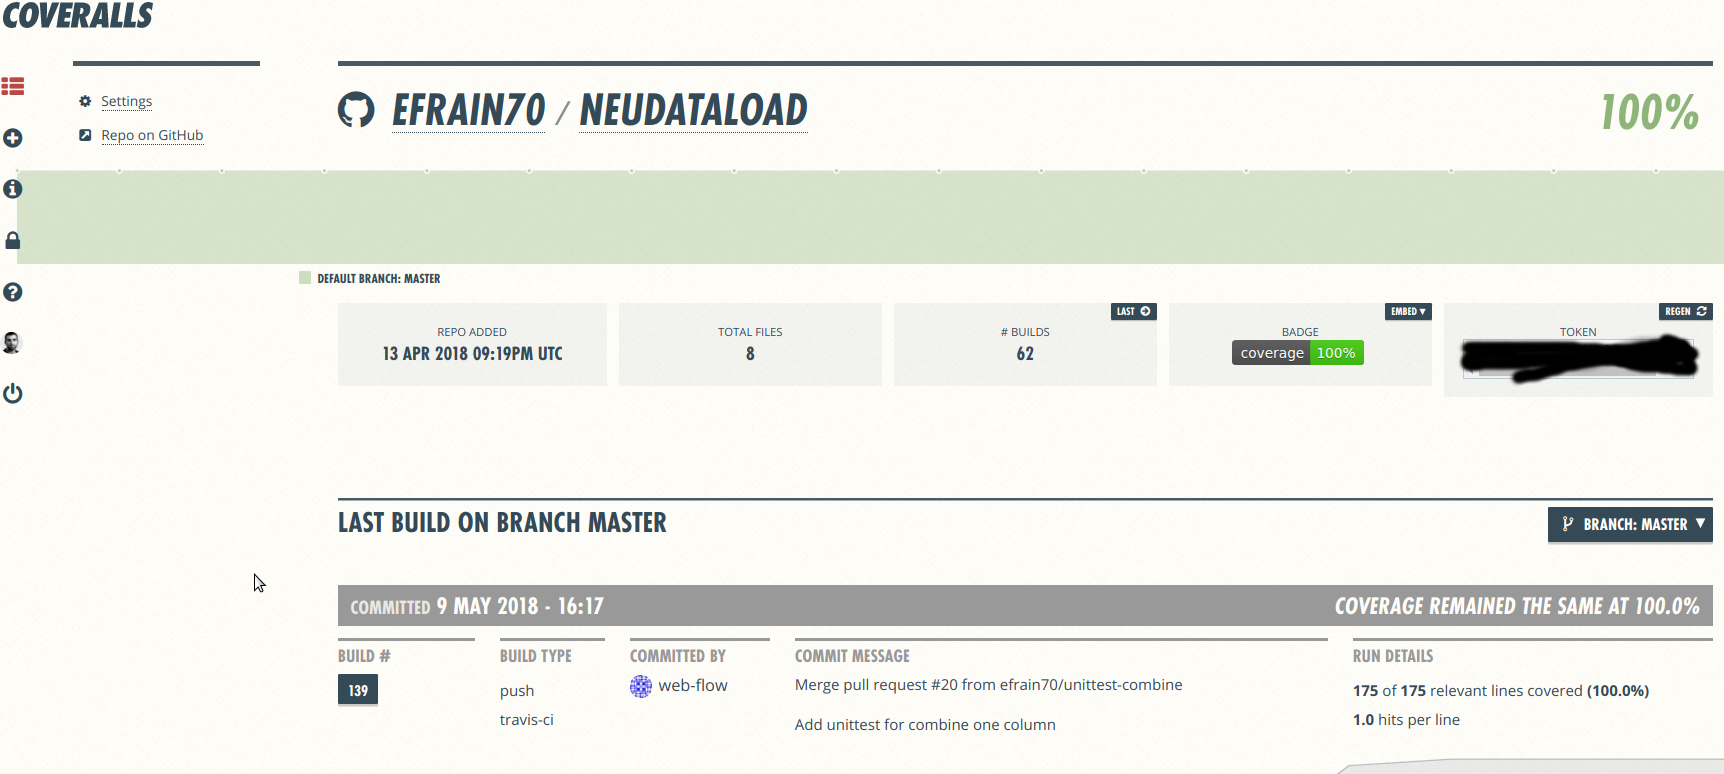
\includegraphics[width=0.8\textwidth]{figs/software/HFRiU5.png}
\caption{Captura de pantalla del proyecto NeuLoadData en Coveralls}
\label{figure:coveralls}
\end{figure}

No solamente ha comprobado que el código funciona correctamente, también que su sintaxis se ajusta con los estándares del lenguaje. Para ello se ha validado el estilo de todo el código bajo la guía especial para Python PEP8 \cite{PEPPython.orgb} y para la documentación en código PEP257 \cite{PEPPython.org} y controlado la complejidad del mismo.

Para ejecutar todo estas validaciones de la calidad del software en un entorno ágil, se ha  configurado el proceso siguiendo un enfoque de integración continua, usando para ello pipelines de la plataforma Travis CI \cite{TravisConfidence} (Dirección del proyecto \url{https://travis-ci.org/efrain70/NeuDataLoad}, imagen \ref{figure:travis}) como plataforma coordinada con el repositorio Github. Esto implica que cada vez que se publique alguna modificación en el código, Github se coordina con Travis CI para la ejecución de todas las pruebas anteriormente descritas reportando los posibles errores automáticamente.

\begin{figure}[H]
\centering
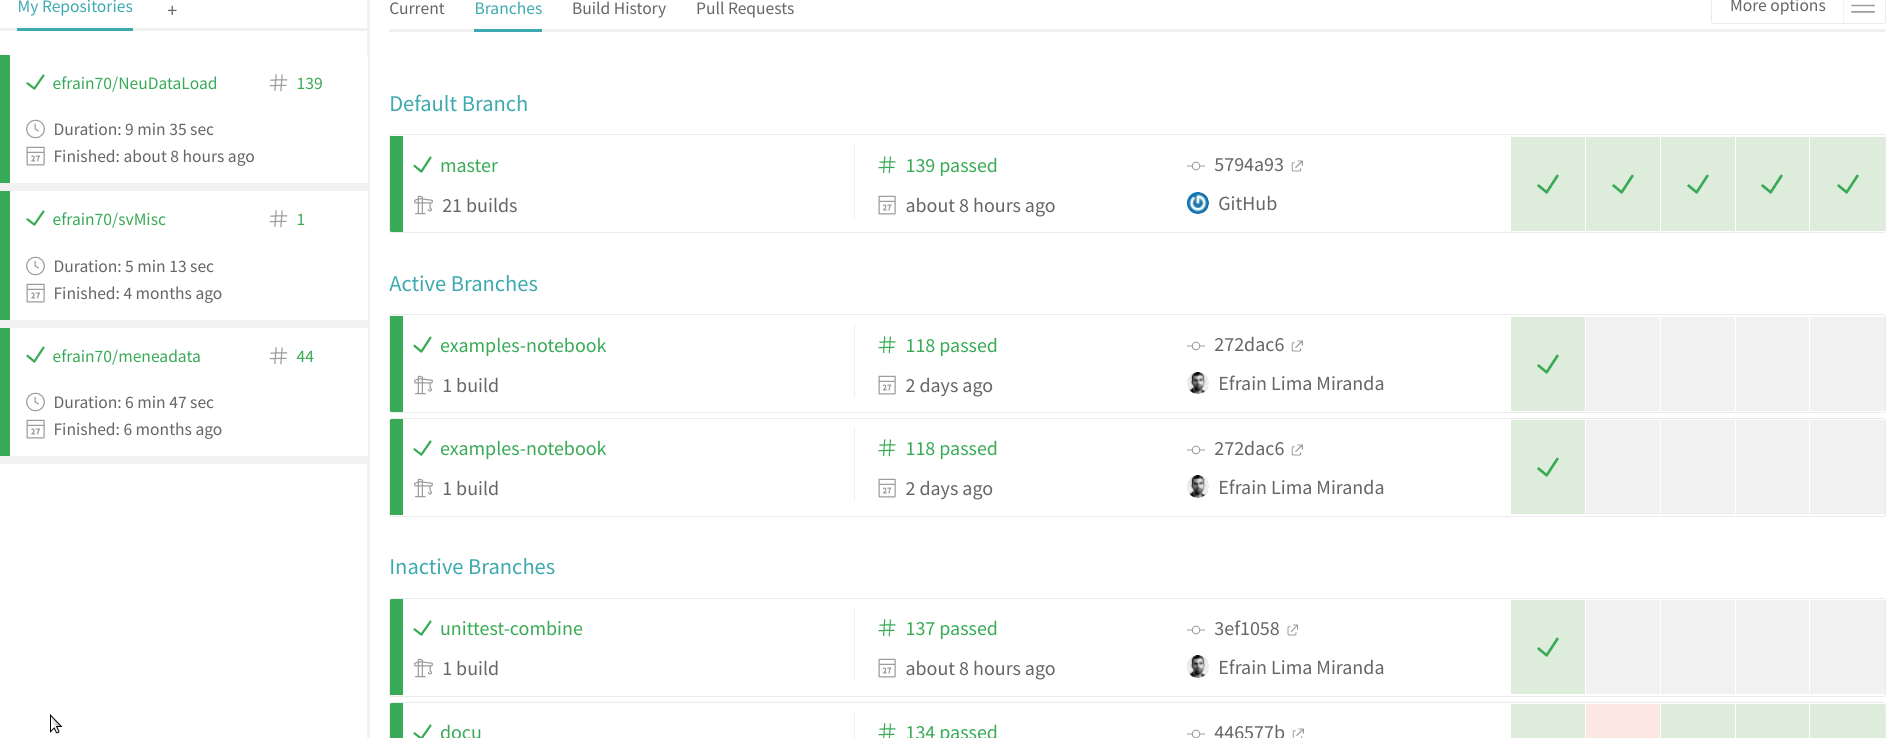
\includegraphics[width=0.8\textwidth]{figs/software/travis.png}
\caption{Captura de pantalla de la ejecución en Travis CI del proyecto NeuLoadData}
\label{figure:travis}
\end{figure}

\subsection{Documentación}
Toda la documentación de este software se ha descrito usando la tecnología propia del lenguaje de Python. Gracias a la utilidad de Sphinx \cite{OverviewDocumentation} se han generado automáticamente la documentación con el contenido descrito en el código. Toda esta documentación del software se ha incluido en el código y generado en formato web para su publicación en Github Pages \cite{GitHubLive.}. Bajo la dirección \url{https://efrain70.github.io/NeuDataLoad/}, imagen \ref{figure:documentacion}, se encuentra la interfaz de la aplicación detallada.

\begin{figure}[H]
\centering
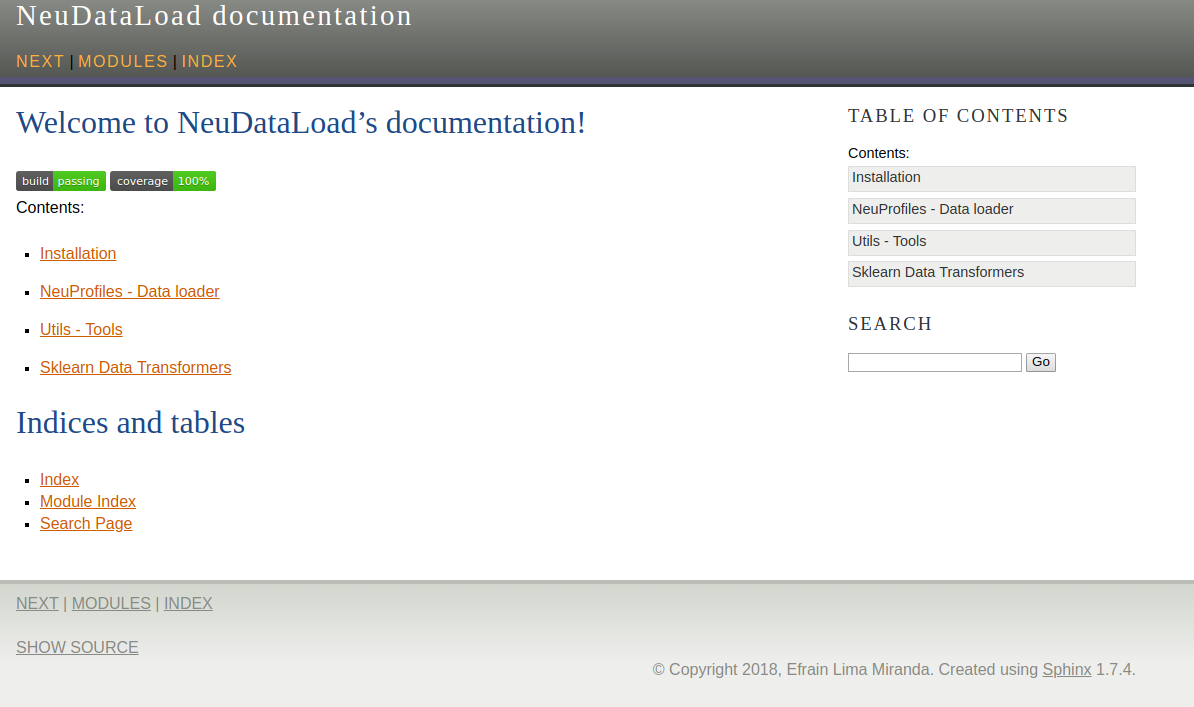
\includegraphics[width=0.8\textwidth]{figs/software/docu.png}
\caption{Captura de pantalla de la documentación en linea de NeuLoadData}
\label{figure:documentacion}
\end{figure}

\subsection{Funcionalidades principales}
Las funcionalidades principales implementadas en software son:

\subsubsection{Aplicación de transformaciones a las matrices}
Para adaptarse a las necesidades de los algoritmos de aprendizaje automático y para mejorar su rendimiento se incluyen un conjunto de herramientas para la transformación de las matrices:

\paragraph{Combinación de las matrices:}
Teniendo como entrada un conjunto de matrices del mismo tamaño NxM, se le aplica una función a las celdas de todas las matrices situadas en las mismas coordenadas i,j dando como resultado una nueva de tamaño NxM con los resultados de la aplicación de la función.

\paragraph{Aplanamiento o remodelación:}
A partir de una matriz de tamaño NxM, se generan una nueva de una única dimensión con los valores extendidos. Es decir, obtendremos N·M atributos nuevos.

\paragraph{Binarización:} A partir de un valor de frontera, la matriz convierte todos sus valores a 1 y 0 dependiendo si éstos superan el valor de frontera. Es decir, se obtiene una matriz con valores binarios de tamaño NxM.

\paragraph{Selección de los atributos:} Selección de atributos del conjunto de datos y de los posibles nuevos atributos generados durante la transformación aplanamiento. 

Todas estas funcionalidades se implementan principalmente en el módulo ‘utils’, pero puede ser usada a través de la clase NeuProfiles directamente o por medio de transformadores de para pipelines de scikit-learn \cite{Scikit-learn:Documentation}. En el módulo transformer están las clases transformadoras (\url{https://efrain70.github.io/NeuDataLoad/transformer.html}) que facilitan la integración en el framefork scikit-learn.

\subsection{Carga automática y validación de las matrices}
Usando través de la ruta local o remota introducida por el usuario, NeuLoadData valida las matrices leídas de los ficheros y las incluye en un único dataframe, contenedor de toda la información de la hoja de cálculos y las matrices de adyacencia.

NeuProfiles es clase que implementa esta funcionalidad a través de su método load, dando como resultado objeto contenedor dataframe de Pandas \cite{PythonLibrary} conjuntamente con las utilidades para la transformaciones de matrices. (\url{https://efrain70.github.io/NeuDataLoad/profiles.html})

